\documentclass[letterpaper,11pt]{article}
\oddsidemargin -1.0cm \textwidth 17.5cm

\usepackage[utf8]{inputenc}
\usepackage[activeacute,spanish, es-lcroman]{babel}
\decimalpoint
\usepackage{amsfonts,setspace}
\usepackage{amsmath}
\usepackage{amssymb, amsmath, amsthm}
\usepackage{comment}
\usepackage{float}
\usepackage{amssymb}
\usepackage{dsfont}
\usepackage{anysize}
\usepackage{multicol}
\usepackage{enumerate}
\usepackage{graphicx}
\usepackage[left=1.5cm,top=2cm,right=1.5cm, bottom=1.7cm]{geometry}
\setlength\headheight{1.5em} 
\usepackage{fancyhdr}
\usepackage{multicol}
\usepackage{hyperref}
\usepackage{wrapfig}
\usepackage{subcaption}
\usepackage{siunitx}
\usepackage{cancel}
\usepackage{mdwlist}
\usepackage{svg}
\pagestyle{fancy}
\fancyhf{}
\renewcommand{\labelenumi}{\normalsize\bfseries P\arabic{enumi}.}
\renewcommand{\labelenumii}{\normalsize\bfseries (\alph{enumii})}
\renewcommand{\labelenumiii}{\normalsize\bfseries \roman{enumiii})}


\begin{document}

\fancyhead[L]{\itshape{Facultad de Ciencias F\'isicas y Matem\'aticas}}
\fancyhead[R]{\itshape{Universidad de Chile}}
\rfoot[]{pág. \thepage}

\begin{minipage}{11.5cm}
    \begin{flushleft}
        \hspace*{-0.6cm}\textbf{FI1000-1 Introducción a la Física Clásica}\\
        \hspace*{-0.6cm}\textbf{Profesor:} Ignacio Bordeu\\
        \hspace*{-0.6cm}\textbf{Auxiliares:} Alejandro Cartes \& Simón Yáñez\\
        \hspace*{-0.6cm}\textbf{Ayudante:} Javier Cubillos\\
    \end{flushleft}
\end{minipage}

\begin{picture}(2,3)
    \put(366, 10){
\includegraphics[scale=0.9]{2020-1/Imágenes/logo/dfi-fcfm.pdf}}
\end{picture}

\begin{center}
	\LARGE\textbf{Auxiliar \#14}\\
	\Large{Repaso C3}
\end{center}

\vspace{-1cm}
\begin{enumerate}\setlength{\itemsep}{0.4cm}

\item[]

\item Un bloque de masa $m$ con un resorte pegado descansa sobre una superficie horizontal sin fricción. El resorte posee constante elástica $k$ y largo del resorte relajado $L$ con masa despreciable. Un segundo bloque de masa $m$ se mueve horizontalmente con velocidad constante $v_0$ y colisiona con el resorte como se muestra en la figura. ¿Cuál es el largo mínimo del resorte durante la colisión?

\begin{figure}[H]
    \centering
    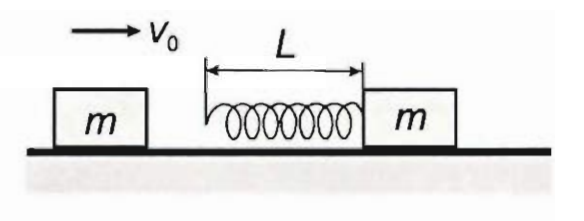
\includegraphics[width = 0.6\textwidth]{2023-1/img/aux_14/Aux 14 - P1.PNG}
    %\caption{Figura P1}
    \label{fig:enter-label}
\end{figure}

\item Tal como se muestra en la figura, una semiesfera de radio $R$ está acoplada sobre un carro simétrico que puede rodar suavemente sobre el suelo horizontal. La masa total del carro es M distribuida homogéneamente, y está inicialmente en reposo. Una bola de masa $m$ descrita puntualmente es liberada tangencialmente en la semiesfera desde un punto h = R sobre su borde. La pelota se desliza sobre toda la semiesfera con fricción despreciable.
\begin{enumerate}
    \item ¿Dónde estará la bola cuando alcance la altura máxima durante su movimiento?
    \item Determine la fuerza con que la bola presiona la semiesfera en su punto más bajo.
\end{enumerate}

\begin{figure}[H]
    \centering
    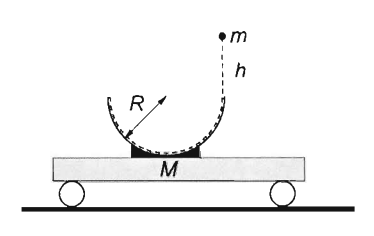
\includegraphics[width = 0.6\textwidth]{2023-1/img/aux_14/Aux 14 - P2.PNG}
    %\caption{Figura P2}
    \label{fig:enter-label}
\end{figure}

\newpage

\item Una argolla de masa $m_1$ que se mueve con rapidez $v_0$ (desconocida), se adhiere a una argolla de masa $m_2$ unida a un bloque de masa $M$ mediante un resorte de constante elástica $k$ y largo natural $L_0$. Inicialmente, la argolla $m_2$ está en reposo y el resorte se encuentra en posición vertical y en su largo natural. El bloque descansa sobre una superficie horizontal rugosa. A consecuencia de la colisión, las argollas continúan moviéndose juntas hasta detenerse cuando el resorte forma un ángulo $\theta$ con la vertical.
    

\begin{enumerate}
    \item Determine la velocidad $v_0$ de la argolla $m_1$
    \item \textbf{[Propuesto]} Determine el coeficiente de roce estático $\mu$ para que el bloque $M$ no resbale durante el movimiento de las argollas 
\end{enumerate}
    
\begin{figure}[H]
    \centering
    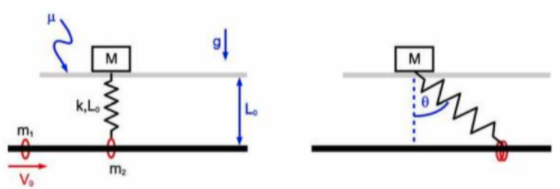
\includegraphics[width=0.6\textwidth]{2021-2/img/aux11/aa.PNG}
\end{figure}



% Para imágenes vectoriales -> el texto tiene que estar en LaTeX
% \begin{figure}[htbp]
%   \centering
%   \svgpath{../Imagenes/ejercicios}  -> .. irse pa'trás 
%   \includesvg{ej5.svg}
% \end{figure}

\end{enumerate}
\end{document}